\begin{ledgroupsized}[r]{120mm}
\footnotesize 
\pstart
\noindent\textbf{\"{U}berlieferung:}
\pend
\end{ledgroupsized}
\begin{ledgroupsized}[r]{114mm}
\footnotesize 
\pstart \parindent -6mm
\makebox[6mm][l]{\textit{L}}Aufzeichnung: LH XXXVII 5 Bl. 6-7. 1 Bog. 4\textsuperscript{o}. \nicefrac{1}{4} S. Die Rechnungen sind gegenl\"{a}ufig im mittleren bis oberen Bereich von Bl. 7~r\textsuperscript{o} verfasst worden; dar\"{u}ber weitere gegenl\"{a}ufig verfasste Rechnungen (Cc 2, Nr. 945 D), die keinen unmittelbar erkennbaren Zusammen\-hang mit N. 33 aufweisen
(sie werden in \textit{LSB} VII ediert).
Der untere Bereich von Bl.~7~r\textsuperscript{o} sowie Bl.~7~v\textsuperscript{o} sind leer;
Bl. 6 überliefert einen Teil von N.~32.
Der Bogen wurde durch Papier\-er\-haltungsmaßnahmen gesichert.
Ein Wasserzeichen in der Mitte.
 \\Cc 2, Nr. 945 E \pend
\end{ledgroupsized}

%\normalsize
\vspace*{5mm}
\begin{ledgroup}
\footnotesize 
\pstart
\noindent\footnotesize{\textbf{Datierungsgr\"{u}nde}: Bl. 6-7 bilden einen Bogen; Bl. 6 geh\"{o}rt zum St\"{u}ck N. 32. Die Rechnungen in N.~33 weisen zudem inhaltliche \"{A}hnlichkeit mit denjenigen auf, die im St\"{u}ck N. 31\textsubscript{2} vorkommen. Sowohl N. 32 als auch N. 31\textsubscript{2} sind eigenh\"{a}ndig auf April 1675 datiert. Es erweist sich daher als plausibel, die gleiche Datierung auch f\"{u}r N. 33 zu \"{u}bernehmen.}
\pend
\end{ledgroup}

\vspace*{8mm}
\count\Bfootins=1500
\count\Afootins=1500
\count\Cfootins=1500
\pstart \noindent
\normalsize
[7~r\textsuperscript{o}] $\rule[-4mm]{0mm}{10mm}\displaystyle ax \, \sqcap \, y^2$. 
Ergo $\rule[-4mm]{0mm}{10mm}\displaystyle y \, \sqcap \, \sqrt{\vphantom{ax}} ax$. 
Et $\rule[-4mm]{0mm}{10mm}\displaystyle z \, \sqcap \, \sqrt{ax + a\beta} - \sqrt{\vphantom{ax}} ax$. 
Unde $\rule[-4mm]{0mm}{10mm}\displaystyle z^2 \sqcap \, ax + a\beta - 2\sqrt{ax + a\beta , ax} + ax$ 
sive: $- z^2 + 2ax + a\beta \ \sqcap \ 2\sqrt{a^2x^2 + a^2 \beta x}$. 
Ergo $\rule[-4mm]{0mm}{10mm}\displaystyle z^4 - 4z^2ax - 2a \beta z^2 \, \ovalbox{$+ \, \edtext{4[a^{2}]x^2}{\lemma{$\displaystyle a$}\Bfootnote{\textit{L ändert Hrsg.}}} + 4a^2 \beta x$} \, + a^2\beta^2 \, \sqcap \ \ovalbox{$4a^2x^2 + 4a^2 \beta x$}$ 
et fiet: $a \beta^2 \sqcap \, 4z^2x$. 
Sive $\rule[-4mm]{0mm}{10mm}\displaystyle z \, \sqcap \, \frac{\beta}{2} \sqrt{\vphantom{\mathstrut \frac{a}{x}}} \frac{a}{x}$. 
Sit jam $\displaystyle y \ \sqcap \ a \sqrt{\protect\vphantom{\protect\mathstrut \frac{a}{x}}} \frac{a}{x}$. %PR: Folgende Cfootnote ist jetzt ersatztlos gestrichen:
% \edtext{}{\lemma{$\displaystyle y \ \sqcap \ a \sqrt{\protect\vphantom{\protect\mathstrut \frac{a}{x}}} \frac{a}{x}$}\Cfootnote{Die neuerliche Setzung widerspricht der urspr\"{u}nglichen Setzung $\displaystyle y = \sqrt{ax}$.}}
Ergo $\rule[-4mm]{0mm}{10mm}\displaystyle z \, \sqcap \, a \sqrt{\vphantom{\mathstrut \frac{a}{x}}} \frac{a}{x} \, - \, a \sqrt{\vphantom{\mathstrut \frac{a}{x}}} \! \frac{a}{x + \beta}$. 
Ergo $\rule[-4mm]{0mm}{10mm}\displaystyle z^2 \, \sqcap \ \frac{a^3}{x} - 2a^3 \sqrt{\vphantom{\mathstrut \frac{1}{x}}} \! \frac{1}{x^2 + x\beta} \, + \frac{a^3}{x + \beta}$. 
Ergo $\rule[-4mm]{0mm}{10mm}\displaystyle 2a^3 \sqrt{\vphantom{\mathstrut \frac{1}{x}}} \! \frac{1}{x^2 + x\beta} \, \sqcap \, \frac{a^3}{x} + \frac{a^3}{x + \beta} - z^2$. 
Ergo $\rule[-4mm]{0mm}{10mm}\displaystyle \overset{2}{\ovalbox{$4$}} \ a^6 \frac{1}{x^2 + x\beta} \, \sqcap \, \frac{a^6}{x^2} \, \ovalbox{$\displaystyle + \frac{2a^6}{x^2 + x \beta}$} - \frac{2a^3z^2}{x} + \frac{a^6}{x^2 + 2 \beta x + \beta^2} \edtext{- \frac{2a^3z^2}{x + \beta} + z^4$. 
Rejectis $\displaystyle z^4$,}{\lemma{$\displaystyle -\, \frac{2a^3z^2}{x + \beta} + z^4$}\Bfootnote{\textit{(1)}\ $\displaystyle - \, \frac{2a^6}{x^2 + x\beta} + \frac{a^6}{x^2} + \frac{a^6}{x^2 + 2 \beta x + \beta^2} \ \sqcap \ 0$ quia $\displaystyle \beta \ \sqcap \ 0$. Ergo $\displaystyle - \, 2a^3$ \textit{(2)}\ . Rejectis $\displaystyle z^4$, \textit{L}}}
et reductis omnibus ad communem denominatorem multiplicando per $\rule[-4mm]{0mm}{10mm}\displaystyle x^2 + x \beta , \ x^2 , \ \edtext{x^2 + 2 \beta x + \beta^2$,
fiet calculus paulo prolixior}{\lemma{$\displaystyle x^2 + 2 \beta x + \, \beta^2$,}\Bfootnote{\textit{(1)}\ fiet: $\displaystyle 2a^6, \ \smallfrown  x^2 , \ x^2 + 2 \beta x + \beta^2 \, \sqcap \ a^6, \ x^2 + x \beta , \ x^2 + 2 \beta x + \beta^2,\!, \ - \, 2a^3z^2, \ x, \ x^2 + \beta x , \ x^2 + 2 \beta x + x^2$ \textit{(2)}\ fiet [...] prolixior. \textit{L}}}. Et sic brevique habebitur $\rule[-4mm]{0mm}{10mm}\displaystyle y^2 \, \sqcap \, \frac{a^3}{x}$ \edtext{seu}{\lemma{}\Afootnote{\textit{Oberhalb der Zeile:} $\displaystyle \cancel{y} \protect\underset{l}{x} \, \sqcap \, - \cancel{y}x$\vspace{-6mm}}} \edtext{$\displaystyle y^2 x \, \sqcap \, a^3$, $\displaystyle y^2 l \ \sqcap \, - \, 2y^2 x$. Ergo $\displaystyle l \ \sqcap \, - \, 2x$. Jam $\displaystyle \frac{z}{\beta} \, \sqcap \, \frac{y}{l}$}{\lemma{$\displaystyle y^2 x \, \sqcap \, a^3$,}\Bfootnote{\textit{(1)}\  sive $\displaystyle 2y^2 \cancel{x} \, \sqcap \, - \, y^2 \cancel{x}$. Ergo $\displaystyle 2l \, \sqcap \, - \, y$. Jam $\displaystyle \frac{z}{\beta} \, \sqcap \, \frac{y}{l}$ \textit{ (2) }\ $\displaystyle y^2 l \ \sqcap \, - \, 2y^2 x$ [...] $\displaystyle \frac{z}{\beta} \, \sqcap \, \frac{y}{l}$ \textit{L}}} 
seu $\displaystyle \frac{z}{\beta} \, \sqcap \, \frac{y}{-2x}$. Et $\displaystyle y \, \sqcap \, a \sqrt{\vphantom{\mathstrut \frac{a}{x}}} \frac{a}{x}$. Ergo $\displaystyle z \, \sqcap \, \frac{a \beta}{-2x} \sqrt{\vphantom{\mathstrut \frac{a}{x}}} \frac{a}{x}$ sive $\displaystyle z^2 \sqcap \frac{a^3 \beta^2}{4x^3}$.
% PR: getilgte Fassung des Eintrags (überholt):
% }{\lemma{$\displaystylex^2 , \ x^2 + 2 \beta x + \beta^2$,}\Bfootnote{ \textit{ (1) }\ fiet: $\displaystyle 2a^6, \ \smallfrown  x^2 , \ x^2 + 2 \beta x + \beta^2 \, \sqcap \ a^6, \ x^2 + x \beta , \ x^2 + 2 \beta x + \beta^2,\!, \ - \, 2a^3z^2, \ x, \ x^2 + \beta x , \ x^2 + 2 \beta x + x^2$ \textit{ (2) }\ fiet [...] $\displaystyle a^3$,  \textit{(a)}\ sive $\displaystyle 2y^2 \cancel{x} \, \sqcap \, - \, y^2 \cancel{x}$. Ergo $\displaystyle 2l \, \sqcap \, - \, y$. Jam $\displaystyle \frac{z}{\beta} \, \sqcap \, \frac{y}{l}$ \textit{(b)}\ $\displaystyle y^2 [...] 2x$. Jam [...] $\displaystyle z^2 \sqcap \frac{a^3 \beta^2}{4x^3}$ \textit{ L}}}
Nempe $\rule[-4mm]{0mm}{10mm}\displaystyle z^2 \sqcap \frac{a^3 \beta^2}{4x^3}$. 
Sive erunt \textit{z} \edtext{quadrata}{\lemma{quadrata}\Bfootnote{\textit{erg. L}}} in ratione ipsorum $\rule[-4mm]{0mm}{10mm}\displaystyle x$ reciproca triplicata. 
\pend
\vspace{2em}
\pstart
\noindent
\centering             
 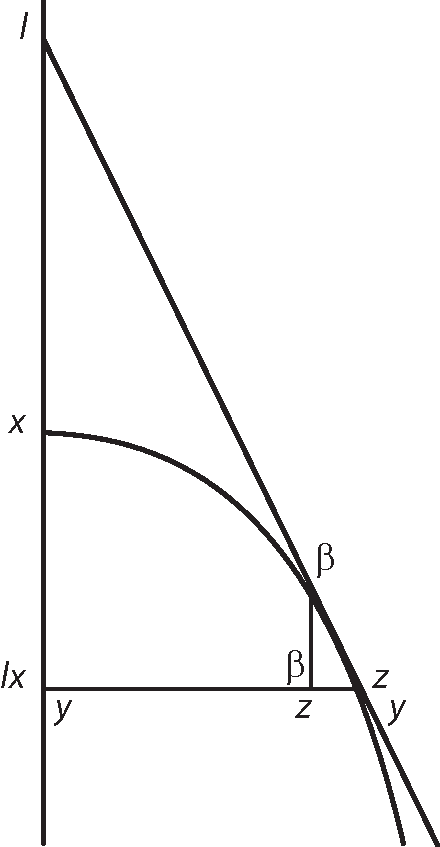
\includegraphics[trim = 0mm -3mm 0mm 0mm, clip,width=0.32\textwidth]{images/lh03705_007r-d1.pdf}\\
 \noindent \centering \setline{1} [\textit{Fig. 1}] %\caption{[\textit{Fig. 1}]}
\pend